\documentclass[12pt]{article}
\usepackage[margin = 1in]{geometry}
\usepackage{amsmath, amssymb, amsthm, graphicx}
\usepackage{enumerate}
\usepackage[all]{xy}
\usepackage{mathrsfs}

%%%%%%%%%%%%%% COLOR COMMENTS! %%%%%%%%%%%%%%%
\usepackage{color}
\newcommand{\dzb}[1]{{\color{blue} \sf
    $\spadesuit\spadesuit\spadesuit$ DZB: [#1]}}
\newcommand{\reword}[1]{{\color{red} \sf $\spadesuit\spadesuit\spadesuit$ reword: [#1]}}

% changed above definition to make comments disappear
%\newcommand{dzb}[1]{}
%\newcommand{reword}[1]{}

% Color names: http://en.wikibooks.org/wiki/LaTeX/Colors#The_68_standard_colors_known_to_dvips
\usepackage[usenames,dvipsnames]{xcolor}
\newcommand{\note}[1]{{\color{BurntOrange} $\blacktriangle\blacktriangle$\sf Note: [#1]}}

\newcommand{\F}[0]{\mathbb{F}}
\newcommand{\tr}[0]{\operatorname{tr}}
\newcommand{\wt}[1]{\widetilde{#1}}
\newcommand{\frob}[0]{\operatorname{Frob}}
\newcommand{\card}[0]{\#}
\newcommand{\pmat}[4]{\begin{pmatrix}#1 & #2 \\ #3 & #4\end{pmatrix}}
\newcommand{\pderiv}[2]{\frac{\partial #1}{\partial #2}}
\newcommand{\Ov}{\mathcal{O}_{v}}
\newcommand{\Ok}{\mathcal{O}_{K}}
\newcommand{\Q}{\mathbb{Q}}
\newcommand{\Z}{\mathbb{Z}}
\newcommand{\C}{\mathbb{C}}
\newcommand{\leg}[2]{\left(\frac{#1}{#2}\right)}
\newcommand{\calO}{\mathcal{O}}
\newcommand{\frakp}{\mathfrak{p}}
\newcommand{\frakq}{\mathfrak{q}}
\newcommand{\mf}[1]{\mathfrak{#1}}
\newcommand{\nm}{\operatorname{N}_{K/\Q}}
\newcommand{\Cl}{\operatorname{Cl}}
\newcommand{\oo}{\mathcal{O}}
\newcommand{\sgn}{\operatorname{sgn}}
\newcommand{\Gal}{\operatorname{Gal}}
\newcommand{\cl}{\overline}
\newcommand{\mc}[1]{\mathcal{#1}}
\newcommand{\Cc}{\mathcal{C}}
\newcommand{\Dc}{\mathcal{D}}
\newcommand{\raym}{\mathcal{C}^{\frakm}_K}
\newcommand{\frakr}{\mathfrak{r}}
\newcommand{\Spec}{\text{Spec} \ }
\newcommand{\Hom}{\text{Hom}}
\newcommand{\ord}{\text{ord}}
\newcommand{\scr}[1]{\mathscr{#1}}
\newcommand{\R}{\mathbb{R}}
\newcommand{\Nm}{\text{Nm}}
\newcommand{\A}{\mathbb{A}}
\newcommand{\ti}{\times}
\newcommand{\Hbb}{\mathbb{H}}
\newcommand{\ol}[1]{\overline{#1}}
\newcommand{\ul}[1]{\underline{#1}}
%\newcommand{\leg}[2]{\left(\frac{ \# 1}{\# 2} \right)}

\DeclareMathOperator{\GL}{GL}
\DeclareMathOperator{\SL}{SL}
\DeclareMathOperator{\Frob}{Frob}
\DeclareMathOperator{\ab}{ab}
\DeclareMathOperator{\cyc}{cyc}
\DeclareMathOperator{\N}{N}
\DeclareMathOperator{\Ver}{Ver}
\DeclareMathOperator{\Art}{Art}
\DeclareMathOperator{\Spl}{Spl}
\DeclareMathOperator{\sep}{sep}
\DeclareMathOperator{\Stab}{Stab}
\DeclareMathOperator{\Sp}{Sp}
\DeclareMathOperator{\SO}{SO}
\DeclareMathOperator{\SU}{SU}
\DeclareMathOperator{\PGL}{PGL}
\DeclareMathOperator{\Mat}{Mat}
\DeclareMathOperator{\Tr}{Tr}
\DeclareMathOperator{\End}{End}
\DeclareMathOperator{\Ad}{Ad}
\DeclareMathOperator{\Aut}{Aut}
\DeclareMathOperator{\argmax}{argmax}
\DeclareMathOperator{\E}{E}


\newtheorem{thm}{Theorem}
\newtheorem{lemma}[thm]{Lemma}
\newtheorem{defn}[thm]{Definition}
\newtheorem{prop}[thm]{Proposition}
\newtheorem{cor}[thm]{Corollary}
\newtheorem{ex}[thm]{Example}
\newtheorem{crit}[thm]{Criterion}


\theoremstyle{remark}
\newtheorem{rem}[thm]{Remark}

\makeatletter
\def\imod#1{\allowbreak\mkern5mu({\operator@font mod}\,\,#1)}
\makeatother

\widowpenalty=1000
\clubpenalty=1000

\title{CS181 Assignment 5}
\author{Ashok Cutkosky and Tony Feng}


\begin{document}
\maketitle

\subsection*{Problem 1.} (a) We fix the following notation for the probability distribution and the utility function. 
\begin{itemize}
\item Let $p_t$ denote the probability distribution upon pursuing target $t$, so $p_t(r)$ is the probability of scoring $r$ points, conditioned on aiming for target $t$. 
\item Let $U(r, s)$ denote the utility from scoring $r$ points given current score $s$. 
\end{itemize} 
Now, given current score $s$, the expected utility from pursuing target $t$ is 
\[
\E(t,s) = \sum_r p_t(r) U(r,s).
\]
Therefore, the optimal action is to aim for target $t^*$ satisfying 
\[
t^* = \displaystyle\argmax_t \E(t,s) = \argmax_t \sum_r p_t(r) U(r,s).
\]
(b) This utility function leads to very greedy play, in which the agent will always aim to score as many points as possible without overshooting the goal. We think it is a pretty good heuristic, but not optimal because the agent will tend to get stuck with a low score, at which point it must try for very particular values that it will hit with low probability. 

We expect an agent playing with this utility function to do well at the beginning of the game, and quickly cut down its score. However, as discussed above, this greedy utility function seems like it would tend to perform poorly at the end, when it must account for subtle considerations like the best small score value to land on. To use an analogy, this strategy is like a golfer who puts all his or her emphasis on driving, and none on putting. \\

\subsection*{Problem 2.} (a) The states are the various score values one can obtain, since we expect our policies should depend on nothing other than our current score. Thus the states are the numbers from $0$ to the maximum score value. The actions are the different throws we can attempt to make (i.e. targets to aim for). Thus the actions are the different areas of the dartboard, as marked above.\\

\noindent (b) The reward for state $0$ is $1$ and the reward for any other state is $0$. This tells our dart robot that the ``winning'' state, $0$, is desirable while any other state is not particularly helpful. Thus we'd expect the robot to attempt to reach the winning state via a path that goes through a minimum number of non-winning states - that is, it will attempt to spend as much time in the winning state as possible.

The discount factor modulates the robot's aggressiveness. It tells the robot how important marginal differences in paths to the winning state are as these paths get longer. The net result is that a high discount factor causes the robot to  emphasize the ``best cases,'' because it weights short games more heavily, while a low discount factor causes the robot to emphasize the ``worst case,'' because it suffers comparatively more from extended games. 

For example, let $\gamma_1$ and $\gamma_2$ be two paths to the winning state. Suppose $\gamma_2$ is one step longer than $\gamma_1$. Then with a low discount factor the robot will see very little difference between $\gamma_1$ and $\gamma_2$ if they are both reasonably long. With a high discount factor the robot will prefer $\gamma_1$ much more that $\gamma_2$. \\

\noindent (c) Constructed. \\

\noindent (d) In the finite horizon case the robot is limited to looking only some constant number of moves ahead. For the darts game the number of moves needed to reach a winning state is not bounded above. We need an infinite horizon to guarantee that the play is coherent for all possible outcomes. 

Another advantage is that this approach is more generalizable. In particular, as we scale the size of the board and the starting score this number increases. If the robot needs $N$ throws to win and has a finite horizon of $M<N$, then the robot is incapable of determining a path from its current state to the winning state. If we have an infinite horizon, on the other hand, the robot will always be able to see such paths and choose an optimal one.\\

\noindent (e) An optimal policy is

\begin{tabular}{c|cc}
State&Ring&Wedge\\
\hline
0&Outer Ring&3\\
1&First Patch&1\\
2&First Patch&2\\
3&Middle Ring&3\\
4&First Patch&4\\
5&Inner Ring&4\\
6&Middle Ring&2\\
7&Center&2\\
8&Outer Ring&4\\
9&Middle Ring&3
\end{tabular}

At high scores, the robot generally attempts to lower the score as much as possible in order to reach $0$ as soon as possible. At low scores, it sometimes deviates from this in order to not get stuck at certain scores. That is more or less the intuition we expected.

(f) As the discount factor changes, the robot still attempts to aim for squares that quickly reduce its score. However, for low discount factors the robot tends to go for more conservative moves - ones that are more likely to minimize its worst-case performance, whereas for high discount factors the robot tends to be more aggressive. This makes sense because the the high discount factor makes differences in time-to-win more important.\\




\subsection*{Problem 3.}(a) If PolicyIteration converges to $\pi$, then setting $\pi = \pi^{\text{new}} = \pi^{\text{old}}$ in the algorithm (p.6 of Lecture 19), we find
\begin{align*}
V(s) &= R(s, \pi(s)) + \gamma \sum_{s'} P(s' \mid s, \pi(s)) V(s') \\
\pi(s) &= \argmax_a R(s,a) + \gamma \sum_{s'} P(s' \mid s,a) V(s').
\end{align*}
By the second equation, $\pi(s)$ is the $a$ maximizing the expression 
\[
R(s, a) + \gamma \sum_{s'} P(s' \mid s, a) V(s')
\]
so by definition 
\[
V(s) = \max_a \left[ R(s,a) + \gamma \sum_{s'} P(s' \mid s,a) V(s') \right].
\]
These are precisely the Bellman-Ford equations. So we know that $\pi,V$ give a solution to the Bellman-Ford equations. But we also know that the solution is unique, so this must be it. \\

\noindent (b) This is a bit involved, but please read it through!

By definition of $\pi^{(2)}(s)$ as 
\[
\argmax_a Q(s,a) = \argmax_a R(s,a) + \gamma \sum_{s'} P(s' \mid s,a) V(s'),
\]
and $V^{\pi^{(1)}}$ as satisfying the equation 
\[
V^{\pi^{(1)}} (s) = R(s, \pi^{(1)}) + \gamma \sum_{s'} P(s' \mid s, \pi^{(1)} ) V^{\pi^{(1)}}(s')
\]
we have the following inequality for each $s$:
\begin{equation}\label{3eq2}
V^{\pi^{(1)}} (s) \leq R(s, \pi^{(2)}) + \gamma \sum_{s'} P(s' \mid s, \pi^{(2)} ) V^{\pi^{(1)}}(s') 
\end{equation}
We want to show that 
\begin{equation}\label{3eq3}
V^{\pi^{(1)}}(s) \leq V^{\pi^{(2)}}(s) \text{ for each }s.
\end{equation}

Define the affine transformation $T$ on the vector space of values on the states by 
\[
T(V)(s) =  R(s, \pi^{(2)}) + \gamma \sum_{s'} P(s' \mid s, \pi^{(2)} ) V(s).
\]
Then by definition, $V^{\pi^{(2)}}(s)$ is the (unique) fixed vector of $T$. 

\begin{lemma}\label{3lem1}
If $V(s) \leq V'(s)$ for each $s$, then $T(V)(s) \leq T(V')(s)$ for each $s$. 
\end{lemma}

\begin{proof}
Indeed, 
\[
(T(V')-T(V))(s) = \gamma \sum_{s'} P(s' \mid s, \pi^{(2)}) (V'(s) - V(s)) \geq 0
\]
because each $V'(s)-V(s) \geq 0$ and $P(s' \mid s, \pi^{(2)}) \geq 0$. 
\end{proof}

We want to show that 
\begin{equation}\label{3eq3}
V^{\pi^{(1)}}(s)  < V^{\pi^{(2)}} (s)  = R(s, \pi^{(2)}) + \gamma \sum_{s'} P(s' \mid s, \pi^{(2)} ) V^{\pi^{(2)}}(s'). 
\end{equation}

Notice that equation \eqref{3eq2} says that for each $s$, $V^{\pi^{(1)}}(s) \leq T(V^{\pi^{(1)}})(s)$. Therefore, applying Lemma \ref{3lem1} repeatedly, we find 
\[
V^{\pi^{(1)}}(s) \leq T(V^{\pi^{(1)}})(s) \leq T^2(V^{\pi^{(1)}})(s) \leq T^{\circ 3}(V^{\pi^{(1)}})(s) \leq \ldots \leq T^{\circ n}(V^{\pi^{(1)}})(s) \leq \ldots
\]
We claim that this sequence converges to $V^{\pi^{(2)}}(s)$, which will establish \eqref{3eq3} as desired. As mentioned above, $V^{\pi^{(2)}}$ is defined to be a fixed point vector of the operator $T$, so by the contraction mapping theorem, it suffices to show that $T$ is a contraction.

\begin{lemma}
$T$ is a contraction with factor $\gamma < 1$. 
\end{lemma}

\begin{proof}
Indeed, 
\begin{align*}
|(T(V')-T(V))(s)| & = |\gamma \sum_{s'} P(s' \mid s, \pi^{(2)}) (V'(s) - V(s))| \\
&\leq \gamma \sum_{s'} P(s' \mid s, \pi^{(2)}) |V'(s)-V(s)| \\
&\leq \gamma |V'(s)-V(s)|
\end{align*}
because $\sum_{s'} P(s' \mid s, \pi^{(2)}) = 1$. 
\end{proof}

By the above Lemma, and the Contraction Mapping Theorem, 
\[
\lim_{n \rightarrow \infty} T^{\circ n}(V^{\pi^{(1)}}) 
\]
is the unique fixed point of $T$, and is equal to $V^{\pi^{(2)}}$. This completes the proof, by the reasoning discussed above. \\ 

\noindent (c) First note that if $V^{\pi^{(1)}}(s) = V^{\pi^{(2)}}(s)$ for each $s$, then the algorithm will converge. Indeed, if $V$ does not change then $\pi$, which is defined in each step as an $\argmax$ with respect to a function depending only on the states, actions, and $V$, will not change either. 

Otherwise, at each step $\sum_s V^{\pi}(s)$ strictly increases. However, there are only finitely many distinct possibilities for $\pi$, since $\pi$ is a function from the finite set of states $S$ to the finite set of actions $A$, and hence only finitely many distinct possibilities for $V^{\pi}$. Therefore, it can only strictly increase finitely many times, so it converges in finitely many steps. By (a), when it converges, it must return an optimal stationary policy. 

\subsection*{Problem 4} (a) We chose two approaches: an $\epsilon$-greedy approach, and an exploration with exponential decay ( Boltzman ``simulated annealing'')  approach. Here are the graphs for the results. 

First, this is the $\epsilon$ greedy algorithm.
\[
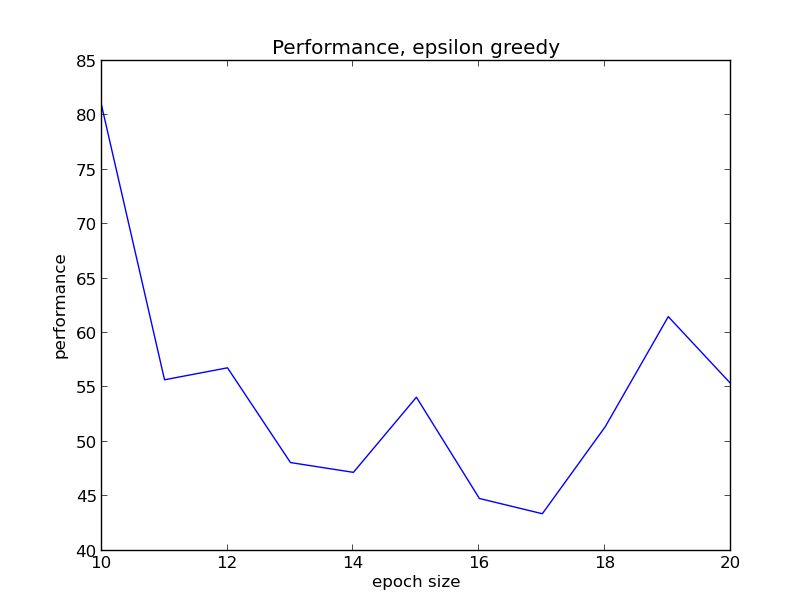
\includegraphics[scale=.8]{epsilon_greedy_performance_modelbased.png}
\]
Second, the simulated annealing algorithm. (Ignore the identical titles. Oops :-))
\[
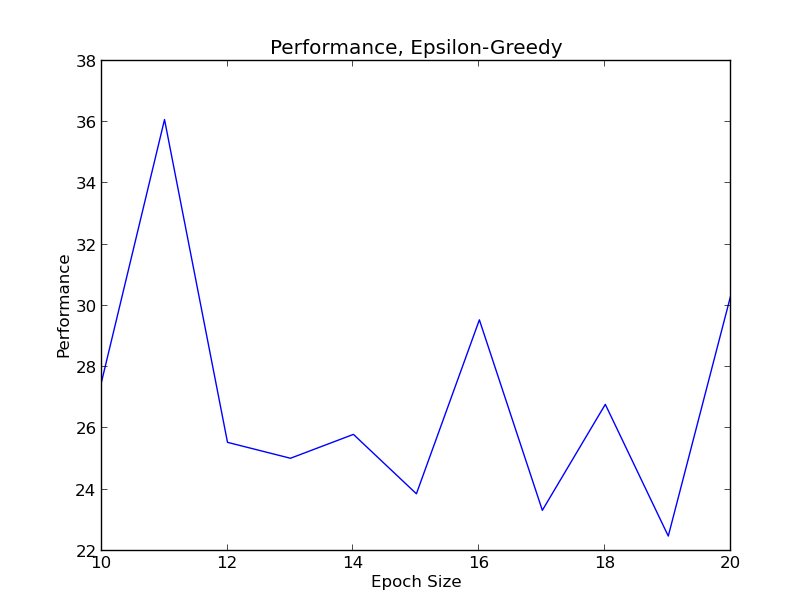
\includegraphics[scale=.8]{simulated_annealing3_performance_modelbased.png}
\]
Simulated annealing performed better. This isn't a huge surprise, since $\epsilon$-greedy is a pretty crude algorithm.\\

\noindent (b) See code. We chose the same strategies as above - $\epsilon$ greedy and simulated annealing. 
\end{document}



